\documentclass[12pt,a4paper]{article}
\usepackage[utf8]{inputenc}
\usepackage{times}
\usepackage{hyperref}
\usepackage{graphicx}
\usepackage{xcolor}
\usepackage{listings}
\usepackage{hyperref}
\usepackage[english]{babel}

\lstset{language=Ruby,keywordstyle={\bfseries \color{blue}}}

\begin{document}
\begin{titlepage}
	\centering
	
\includegraphics[width=0.66\textwidth]{src/title_logo.png}\par\vspace{1cm}
	{\scshape\LARGE Polytech Montpellier\par}
	\vspace{1cm}
	{\scshape\Large WOA Project\par}
	\vspace{1.5cm}
	{\huge\bfseries MenexaTech\par}
	\vspace{2cm}
	{\Large\itshape Yannick Mayeur\par}
	\vfill
	supervised by\par
	Arnaud \textsc{Castelltort}\par
	and\par
	Anne \textsc{Laurent}

	\vfill

% Bottom of the page
	{\large \today\par}
\end{titlepage}

\tableofcontents
\break


\section{Introduction}

When preparing for an exam it is good to know, what the exam may look like, and
what the teacher expects the students to know. Sadly this is not always
possible, because the previous exams of a given course are not always made
available by the teachers or the students that took it. At Polytech in IG a
google drive folder with some old exams exists. This is already very good, but
what would be even better is a place where students could get all of these
resources and also have a place to discuss them. That is how the idea for
MenexaTech was born. MenexaTech is a web application allowing students to
learn in a more effective way. By enabling  them to share previous exams and
offering them a place for discussion.


\section{Presentation of MenexaTech}

MenexaTech allows users, most of which are probably students, to follow or not
a certain number of courses. These courses all have a certain number of old
exams the user can download and each of them has a little forum where users
can discuss there answers.

Some Users are admins, to be an admin you will have to be a class
representative. Admins have the power to create and edit courses, as well as
old exams.


\section{Instructions}

All the instructions to get the project up and running on your machine are
available on the projects README on the GitHub Repository: 
\url{https://github.com/yannick-mayeur/project_app}

\section{Technologies}

\subsection{Description of the technologies}

\subsubsection{Ruby on Rails}
To develop my web application I choose to use the Rails framework.
Rails is running on the Ruby programming language. Rails being a mature
framework, countless resources to help get started are available. The framework
once taken in hand helps build REST compliant applications more easily. One
of its design paradigms is "convention over configurations". This appealed to
me a lot because configuring something you do not entirely understand is always very
hard, and takes a lot of time. Moreover, Rails is easily testable with unit and
integration tests. This is very good to be sure no new functionality breaks
another part of the application.

\begin{figure}[h]
   \centering
   
\includegraphics[scale=0.1]{src/rails_logo.png}
   \caption{\label{fig:rlogo} Ruby on Rails logo}
\end{figure}


\subsubsection{Bootstrap}

Bootstrap is a front-end library that helps you build good looking applications
easily. Bootstrap has a lot of pre made components you can use in your
applications. Not having a very good eye for design, Bootstrap was the perfect
solution for me.

\begin{figure}[h]
   \centering
   
\includegraphics[scale=0.5]{src/bootstrap_logo.png}
   \caption{\label{fig:blogo} Bootstrap logo}
\end{figure}


\subsubsection{Heroku and Google Cloud Storage}
To deploy my web application I used Heroku. Heroku is a cloud PaaS (Platform as
a Service) which supports Ruby on Rails. Heroku makes it very easy to deploy a
web application due to its numerous build packs. It has a free version which is
easily enough for a small application like MenexaTech in its current state, and
with its current user base. But Heroku also makes it very easy to scale an
application.

I used Google Cloud Storage to host the files of Rails's Active Storage
service. I couldn't just use the local disk of Heroku because it is an
"ephemeral" hard drive, meaning that the data written to it is not persistent.

\begin{figure}[h]
   \centering
   
\includegraphics[scale=0.05]{src/heroku_logo.png}
   \caption{\label{fig:hlogo} Heroku logo}
\end{figure}


\subsubsection{Git and GitHub}
When working on a project it is very important to use a VCS (Version Control
System). This type of tool makes it easy to see what change in the application
produces bugs, and allows the programmer to roll these changes back. Git is the
leading VCS on the market. To make the codebase of MenexaTech available online
I choose to use GitHub. The code being on a public Repository it allows users
to see how the application is build, and maybe even make Pull Requests to fix
some bugs or add new features.

\begin{figure}[h]
   \centering
   
\includegraphics[scale=0.15]{src/github_logo.png}
   \caption{\label{fig:ghlogo} GitHub logo}
\end{figure}


\subsubsection{PostgreSQL}
PostgreSQL is an open-source database management system. It is supported by
Heroku.

\begin{figure}[h]
   \centering
   
\includegraphics[scale=0.3]{src/postgres_logo.png}
   \caption{\label{fig:ghlogo} PostgreSQL logo}
\end{figure}

\subsection{Learning the technologies}

One of the biggest challenges of this project was to learn a lot of new
technologies, and use them as well as possible in short frame of time. I made it
possible by choosing technologies that I thought on one hand would be
interesting for me to know. And on the other hand would offer a community with
a lot of support because they a mature and still very active technologies and
so they come with a great amount of good resources to learn from on the
internet. Git and GitHub are the technologies I was the most familiar with
before diving into this project.  Some of the resources I used to learn are:

\begin{itemize}  
\item Official Rails Guides
\item Ruby On Rails Tutorial (Rails 5): Learn Web development with Rails,
	by Michael Hartl
\item RailsCasts
\item Bootstrap documentation
\item Heroku documentation
\end{itemize}


\section{Architecture of the application}

\begin{figure}[h]
	\centering
	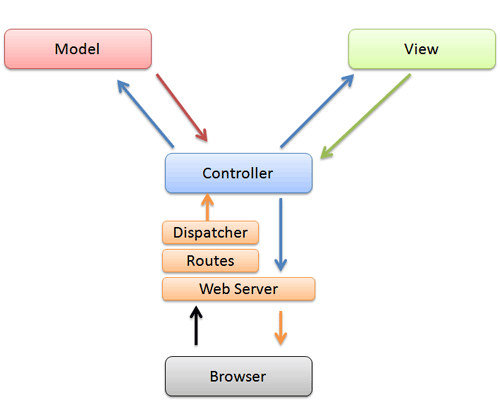
\includegraphics[scale=0.5]{src/mvc.png}
	\caption{\label{fig:mvc} MVC Architechture}
\end{figure}

Model-View-Controller is a very popular design pattern, for designing web
applications. Rails is an MVC framework, so following this architechture was
fairly simple.

In the Rails MVC, when the user makes a request for a page through his web
browser, the URL he ask for is routed to a particular method in a controller.
The job of the controller is to gather all the data from the model that
will have to be used in the view. The view is then created with this data and is
sent back to the browser where the user can see the result. These interactions
can clearly be seen in figure~\ref{fig:mvc} on page~\pageref{fig:mvc}.


\subsection{Pros and Cons}

MVC is good way of creating a web application. It has a very clear design,
which allows for a clean separation of the different parts of the application,
and thus make the application very scalable. However MVC also has some
drawbacks. It sometimes unnecessarily complicates, things that should be simple.


\section{Architecture of the Database}

\begin{figure}[h]
	\centering
	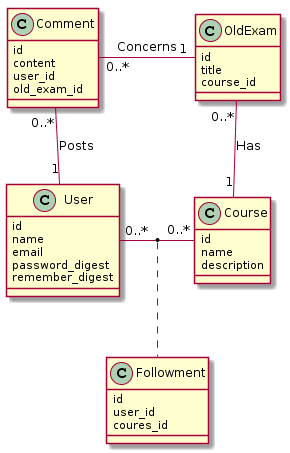
\includegraphics[scale=0.7]{src/digram.png}
	\caption{\label{fig:uml} Class Diagram of the Database}
\end{figure}

We can see in figure~\ref{fig:uml} the different tables of the database and the
relations they have between them.

The database was created though Rails's Active Record Migrations. This feature of
Rails is a convenient way of creating the database, and making it evolve
over time.


\subsection{Description of the database}

The User Table contains all the users of the application. A User is identified
with an id, he also has a name, an email, which he uses to login, a
password\_digest, which is a hashed version of his password, and a
remember\_digest that is used for authentication though cookies.

The Course Table is the cornerstone of the application. A Course like all the
other tables is identified with an id. It also has a name, and a short
description.

The Followment table is where is stored what courses a user follows.
"Followment" is an invented word, to respect the Rails convention of having a
noun as name for Models. It stores the id of the user and of the course
concerned by the follow relationship.

The OldExam table is where the old exams are stored. An OldExam has a title,
and references the course it belongs to. An OldExam also has a file, though the
Active Storage service offered by Rails.

The Comment table is where the comments are stored. A comment has content, it
references the old exam that the comment concerns, and the user that posted the
comment.

\subsection{Pros and Cons}


The principle disadvantage of this model is that all courses are mixed
together. That would be okay if only one class would use the application, but
for more classes the list of courses will probably start to get very cluttered.
A good future improvement would be to add a Class Table to better organize
courses.

One clear advantage would be the use of a table for the follow relationship.
Indeed in Rails there are two ways of doing a many to many relationship. Either
it you use the \lstinline{has_and_belongs_to_many} statement, that uses a table
which is impossible to use to store additional informations. Or can use the
\lstinline{has_many_though} statement which allows you to get your relationship
though a middle table. I went for the latter solution, which offers way more
scalability.


\section{Post Mortem}


\subsection{What went right}

This project was a very good experience. It was a good introduction to web
development and the technologies related to it. It was very exciting to do a
project that had almost no restrictions on the theme and on the technologies to
use.

The project allowed me to see that at the end of IG3 we have some real skills
and that we can build applications that could be used in the real world.

Most of what I initially wanted to put in the application is in it at the end
of the project. I think I managed to organise myself properly and correctly
estimated what would be doable at the beginning of the project. But I got a lot
of new ideas that I have no time to implement. That means that I will probably
continue working on it in my spare time.

\subsection{What went wrong}

Even if in the end all worked out pretty well for my project, some things took me
a lot more time that expected. Logins for example. Programming the application
in a stateless way, sessions were out of question. However most of the
resources I found on the internet advises to use sessions for logins. I had to
patch a lot of different sources together to manage to get what I think is a
secure cookie based authentication.

Another problem I had was with Rails's Active Storage service. I noticed very
late in the development process that Heroku's disk was "ephemeral", meaning
that I had to find a free solution to host the files. Luckily I managed to make
Google Cloud Storage work after countless tries and comprehension problems.

\subsection{Lessons learned}

This project allowed me to learn how to learn new technologies in a more effective
way, the project having to be made in a relatively short amount of time.

I learned that well structuring your code base and using good tools like a VCS
are even more essential than I thought if you don't want to spend a lot of time
finding where a bug comes from or refactoring a chunk of your code.

Well knowing how something was designed helps to build application that will be
scalable. The biggest example I have of that is the REST architectural style
that respect the HTML protocol.


\end{document}
